\subsubsection{„Heritrix“ sistema}
Nepelno siekiančios organizacijos „Internet Archive“ suprojektuotas peržiūros robotas, kurio pagrindinis tikslas rinkti svetainių kopijas ir saugoti jų registrą ateities kartoms. \cite{HeritrixArchitecture}.

\ref{fig:heritrix} schemoje pavaizduota šio roboto architektūra, pasižyminti 3 esminiais komponentais -- operatoriaus konsole (asministratoriaus valdymo sąsaja), peržiūros konfigūratoriumi (peržiūros parametrų nustatymas) ir peržiūros valdikliu (peržiūros proceso koordinavimas) \cite{HeritrixArchitecture}. Sistema nepalaiko išskirstyto tinkle peržiūros koordinavimo \cite{HeritrixArchitecture}, žvalgymas vyksta vienoje fizinėje mašinoje, programa turi daug peržiūros agentų gijų, dirbančių lygiagrečiai \cite{HeritrixArchitecture}. Šioms gijoms duodami žvalgytini URL adresai kitas(URL) operacijos pagalba. Šį koordinavimo procesą atlieka peržiūros valdiklis \cite{HeritrixArchitecture}.
\begin{figure}[htp!]
\hspace{-1cm}
\centering
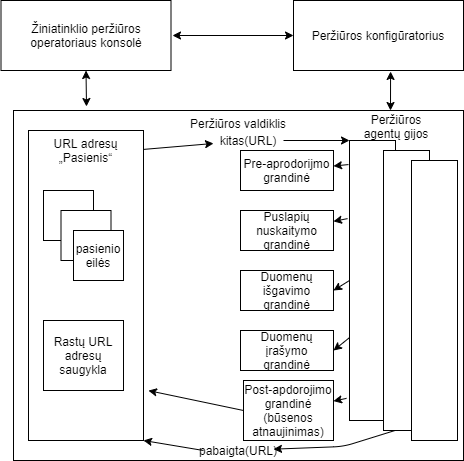
\includegraphics[scale=0.6]{img/heritrix.png}
\caption{„Heritrix“ peržiūros roboto architektūra}
\label{fig:heritrix}
\end{figure}